\documentclass[conference]{IEEEtran}
\IEEEoverridecommandlockouts
\usepackage{cite}
\usepackage{amsmath,amssymb,amsfonts}
\usepackage{algorithm}
\usepackage{algorithmic}
\usepackage{graphicx}
\usepackage{xcolor}
\usepackage{booktabs}
\usepackage{multirow}
\usepackage[hidelinks]{hyperref}

\newcommand{\Ex}{\mathbb{E}}
\newcommand{\todo}[1]{\textcolor{red}{[#1]}}

\begin{document}

\title{Tensor-Network Joint-Loss Models for Multi-Country Catastrophe Bonds: Exact Evaluation Beyond $10^{40}$ States and Born-MPS Loaders for Quantum Amplitude Estimation}

\author{\IEEEauthorblockN{\todo{Author 1}, \todo{Author 2}, \todo{Author 3}}
\IEEEauthorblockA{School of Electrical and Electronic Engineering, Hanoi University of Science and Technology, Hanoi, Vietnam\\
\todo{email}\\
Phase~1 submission --- ADB Quantum Innovation Challenge: Joint-Loss Modelling for Disaster Risk Financing}}

\maketitle

\begin{abstract}
The joint tail of a multi-country catastrophe-bond portfolio is a probability distribution over $10^{n}$ capped
loss states for $n$ countries, which defeats exact enumeration beyond a few countries and makes rare joint events
expensive to sample. We represent this distribution as a matrix product state (MPS), a quantum-inspired tensor
network. For the ADB benchmark (Kyrgyz Republic and Tajikistan) the MPS reproduces all five focus targets in all
five scenarios to within $6\times10^{-8}$ relative error, the residual being a stated Poisson truncation. We then
extend the benchmark to a chain of countries along a shared fault system, in which shared earthquakes hit
\emph{neighbouring} countries. This local dependence has no single common factor, but its three-year term
distribution is an exact MPS with bond dimension 64. Contracting it evaluates every target exactly for 40 countries
($10^{40}$ annual states) in 17\,s on a two-core CPU, for targets as small as $10^{-55}$, which Monte Carlo could
not resolve with $10^{17}$ samples. Tensor-train SVD, applied without knowledge of the model structure, finds ranks of
at most 7 for $p$ and 13 for $\sqrt{p}$ at $10^{-8}$ tolerance, independent of $n$ for $n=3$--$5$. The $\sqrt{p}$
representation is a Born machine that can be prepared on a quantum computer with $4n+\lceil\log_2\chi\rceil$ qubits
and cost linear in $n$, giving a scalable loader for quantum amplitude estimation. We find that state fidelity is a
misleading truncation criterion for tail risk: at $\chi=3$ the infidelity is $6\times10^{-5}$ while the
all-exhausted probability is wrong by $79\%$; $\chi=8$ brings every target within $5\times10^{-6}$.
\end{abstract}

\begin{IEEEkeywords}
tensor networks, matrix product states, quantum-inspired algorithms, Born machine, catastrophe bonds, joint tail risk, quantum amplitude estimation
\end{IEEEkeywords}

%=====================================================================
\section{Introduction}
%=====================================================================
\IEEEPARstart{P}{arametric} catastrophe bonds pay when an objective trigger is met, which makes them fast but makes
their value depend on how triggers co-occur across countries~\cite{brief}. ADB's 2026 disaster relief bonds cover
earthquake and extreme precipitation in the Kyrgyz Republic and Tajikistan~\cite{adbbond}. The challenge
brief~\cite{brief} formalises the portfolio as a distribution over joint outcomes and notes that, with two perils
per country, the annual state space has $10^{n}$ states for $n$ countries: exact enumeration becomes impractical, and
sampling error on joint-tail targets grows.

The brief lists tensor networks among the quantum-inspired methods that may represent joint distributions ``more
faithfully, or with fewer parameters''~\cite{brief}. Matrix product states (MPS), also called tensor trains, express a
tensor with $n$ indices as a chain of small cores~\cite{orus2014,oseledets2011}. They are exact for distributions whose
correlations pass through a bounded number of states across any cut, which is the case for hazards that couple
neighbouring regions. They are also the natural classical counterpart of quantum generative models: an MPS over
$\sqrt{p}$ is a Born machine~\cite{han2018} that a quantum computer can prepare sequentially~\cite{schon2005}.

\subsection{Contributions}
\begin{enumerate}
\item An exact MPS construction of the three-year capped term distribution, validated against the ADB reference
values (Section~\ref{sec:adb}) and brute-force enumeration (Section~\ref{sec:valid}).
\item A chain extension of the benchmark with neighbour-coupled shocks, for which single-factor conditioning
does not apply, evaluated exactly up to $n=40$ (Section~\ref{sec:scale}).
\item Evidence that the joint distribution is intrinsically low-rank: model-agnostic TT-SVD ranks of $p$ and
$\sqrt{p}$ (Section~\ref{sec:ranks}).
\item A Born-MPS loader for quantum amplitude estimation with qubit and CNOT estimates, and the finding that
fidelity does not control tail error (Section~\ref{sec:born}).
\end{enumerate}
This paper complements a companion submission that studies quantum amplitude estimation (QAE) against the ADB
sampling baselines~\cite{paper1}; here the focus is representation and loading.

%=====================================================================
\section{Background}
%=====================================================================
\subsection{The ADB benchmark}
Each country holds a USD~80\,m bond over three years: USD~70\,m for earthquake, paid in quarter steps that
accumulate to the sub-limit, and USD~10\,m for precipitation, paid at most once~\cite{brief}. Earthquake payouts
follow a compound Poisson process fitted to four annual exceedance probabilities; shared events arrive at rate
$c=0.0029667$ per year and draw sizes independently in each country. Precipitation triggers with probability $2\%$
per country, with a shared component of rate $c_r=0.005051$. The term state of country $i$ is $s_i=2a_i+r_i$ with
$a_i\in\{0,\dots,4\}$, $r_i\in\{0,1\}$, and
\begin{equation}
L_i=70\,\text{m}\cdot a_i/4+10\,\text{m}\cdot r_i,\qquad L=\textstyle\sum_iL_i .
\end{equation}
The five targets are $\Ex[L]$, $\Pr(\text{all pay})$, $\Pr(L>T)$, $\Ex[(L-T)^{+}]$ and $\Pr(\text{all exhausted})$, with
$T$ equal to half the total principal (USD~80\,m for $n=2$).

\subsection{Matrix product states}
A tensor $P(s_1,\dots,s_n)$ is an MPS if
\begin{equation}
P(s_1,\dots,s_n)=G_1[s_1]\,G_2[s_2]\cdots G_n[s_n],
\label{eq:mps}
\end{equation}
with $G_i[s_i]$ a $\chi_{i-1}\times\chi_i$ matrix and $\chi_0=\chi_n=1$. Storage and contraction cost are linear in
$n$ and polynomial in the bond dimension $\chi=\max_i\chi_i$. Any tensor can be compressed by TT-SVD to a prescribed
Frobenius tolerance, which reveals its ranks without prior knowledge of its structure~\cite{oseledets2011}.

%=====================================================================
\section{Model: Neighbour-Coupled Countries}\label{sec:model}
%=====================================================================
We place $n$ countries on a chain, alternating the Kyrgyz and Tajik parameters, and attach a shared-earthquake
process of rate $c$ to every link $(i,i+1)$. Each country keeps its total earthquake rate $\Lambda_i$, so its
idiosyncratic rate is $\Lambda_i-d_ic$, with $d_i\in\{1,2\}$ its number of links. A global shared-precipitation shock
of rate $c_r$ hits every country. For $n=2$ the chain has one link and the model is exactly the ADB benchmark.

Let $K_{i,y}\sim\mathrm{Poisson}(c)$ be the number of shared events on link $i$ in year $y$, truncated at $K\le3$
(probability mass lost $\approx c^{4}/24=3\times10^{-12}$ per link-year). Because shared events draw sizes
independently per country, country $i$ depends on the links only through $k_{i-1,y}+k_{i,y}$. Given the link counts
and the rain pattern $J=(J_1,J_2,J_3)$, the countries are independent, and the term distribution is
\begin{equation}
P(s)=\sum_{J}w_J\!\!\sum_{\{k_{i,\cdot}\}}\prod_{i=1}^{n-1}\omega(k_{i,\cdot})\prod_{i=1}^{n}\pi_i\!\left(s_i\,\middle|\,k_{i-1,\cdot}+k_{i,\cdot},J\right),
\label{eq:chain}
\end{equation}
where $k_{i,\cdot}=(k_{i,1},k_{i,2},k_{i,3})$, $\omega$ is the product of Poisson weights over the three years, and
$\pi_i$ is the capped sum of three annual local distributions. Equation~\eqref{eq:chain} is an MPS of the
form~\eqref{eq:mps} for each of the eight rain patterns $J$: the bond on link $i$ is indexed by $k_{i,\cdot}$, which
takes $4^{3}=64$ values, and
\begin{equation}
G_i[s_i]_{\alpha\beta}=\pi_i\!\left(s_i\,\middle|\,\alpha+\beta,J\right)\omega(\beta).
\end{equation}
No single latent variable separates all countries, so the single-factor conditioning used in the companion
paper~\cite{paper1} does not apply; its natural generalisation would enumerate $64^{n-1}$ link configurations.

%=====================================================================
\section{Method}\label{sec:method}
%=====================================================================
\subsection{Exact contraction of the targets}
Products of per-site functions contract in one sweep: with $v_i(s)=\mathbf{1}[s>0]$ (all pay) or
$\mathbf{1}[s=9]$ (all exhausted), $\sum_sP(s)\prod_iv_i(s_i)=\prod_i\big(\sum_{s_i}G_i[s_i]v_i(s_i)\big)$. Expected loss
uses a two-component environment that carries the marginal and the first moment. Sum-dependent targets carry the
partial loss $\ell$ in USD~2.5\,m units through the sweep (Algorithm~\ref{alg:contract}). The cost is
$O(n\cdot10\cdot\chi^{2}\cdot\ell_{\max})$ with $\ell_{\max}=32n$, i.e.\ $O(n^{2}\chi^{2})$, against $O(10^{n})$
for enumeration.

\begin{algorithm}[t]
\caption{Exact loss distribution by MPS contraction}
\label{alg:contract}
\begin{algorithmic}[1]
\REQUIRE cores $G_1,\dots,G_n$; unit losses $u(s)=7\lfloor s/2\rfloor+4(s\bmod2)$
\STATE $E[\cdot,\ell]\leftarrow\delta_{\ell,0}$ \COMMENT{environment: bond $\times$ partial loss}
\FOR{$i=1$ \TO $n$}
  \STATE $E'\leftarrow0$
  \FOR{$s=0$ \TO $9$}
    \STATE $E'[\beta,\ell+u(s)]\mathrel{+}=\sum_\alpha E[\alpha,\ell]\,G_i[s]_{\alpha\beta}$
  \ENDFOR
  \STATE $E\leftarrow E'$
\ENDFOR
\RETURN loss pmf $D(\ell)=E[1,\ell]$; then $\Pr(L>T)$ and $\Ex[(L-T)^{+}]$
\end{algorithmic}
\end{algorithm}

\subsection{Model-agnostic rank discovery}
To test whether low rank is a property of the distribution rather than of our construction, we form the full
tensor for $n=3$--$5$ and apply TT-SVD~\cite{oseledets2011} to $p$ and to $\sqrt{p}$ at tolerances $10^{-4}$ and
$10^{-8}$.

\subsection{Born-MPS loader for QAE}\label{sec:bornmethod}
QAE needs an oracle that prepares $\sum_s\sqrt{p(s)}\lvert s\rangle$~\cite{brassard2002,montanaro2015}. If
$\sqrt{p}$ is an MPS of bond $\chi$, the state can be prepared by a sequence of $n$ unitaries, each acting on one
four-qubit site register and a $\lceil\log_2\chi\rceil$-qubit bond register that returns to $\lvert0\rangle$ at the end~\cite{schon2005}.
The loader therefore needs $4n+\lceil\log_2\chi\rceil$ qubits. Bounding each site unitary by the generic
$\tfrac{23}{48}4^{q}$ CNOT count for $q$ qubits~\cite{shende2006} gives a per-site cost independent of $n$. Because the
loader prepares the \emph{term} state directly, the year-by-year adders of the companion construction~\cite{paper1} are
not needed. We truncate $\sqrt{p}$ by TT-SVD at fixed $\chi$, square, renormalise, and measure both state infidelity
and the relative error of every target.

%=====================================================================
\section{Results}\label{sec:results}
%=====================================================================
\subsection{ADB benchmark reproduction}\label{sec:adb}
For $n=2$ the MPS contraction reproduces the exact targets of all five scenarios (Table~\ref{tab:adb}). The largest
relative deviation, $6.0\times10^{-8}$ in \texttt{common-shock}, comes from the Poisson truncation at $K\le3$, which
matters most when the shared rate is doubled; the \texttt{independent} scenario, which has no shared events, matches
to machine precision. Each evaluation takes 0.02\,s.

\begin{table}[t]
\caption{MPS contraction versus exact ADB values ($n=2$)}
\label{tab:adb}
\centering\footnotesize
\setlength{\tabcolsep}{2.2pt}
\begin{tabular}{lrrrrrr}
\toprule
Scenario & $\Ex[L]$ & pay & $L\!>\!80$m & stop & exh. & max rel.\\
 & USD m & \% & \% & USD & \% & dev.\\
\midrule
base & 10.06 & 4.414 & 1.205 & 282{,}355 & 0.0032 & $5.2\times10^{-9}$\\
independent & 10.06 & 2.716 & 0.719 & 171{,}266 & 0.0004 & $<10^{-15}$\\
common-shock & 10.06 & 5.053 & 1.607 & 385{,}043 & 0.0044 & $6.0\times10^{-8}$\\
rain-stress & 11.17 & 7.046 & 1.322 & 306{,}286 & 0.0069 & $5.2\times10^{-9}$\\
rain-cover & 9.97 & 4.414 & 0.700 & 170{,}927 & 0.0032 & $5.2\times10^{-9}$\\
\bottomrule
\end{tabular}
\end{table}

\subsection{Validation against enumeration}\label{sec:valid}
For the chain model with $n=3$ and $n=4$ we contract the MPS to the full $10^{n}$-entry tensor and compute every
target by direct summation. Algorithm~\ref{alg:contract} agrees to $5.7\times10^{-16}$, and the total probability is
$1-2\times10^{-11}$, consistent with the truncation.

\subsection{Scaling}\label{sec:scale}
Table~\ref{tab:scale} reports exact targets and runtime for chains of up to 40 countries. Runtime grows roughly
linearly in $n$ and stays below 20\,s at $n=40$, where the annual state space has $10^{40}$ states. The probability
deficit grows to $3.8\times10^{-10}$, consistent with $3(n-1)$ truncated link-years.

\begin{table}[t]
\caption{Exact chain targets by MPS contraction}
\label{tab:scale}
\centering\small
\setlength{\tabcolsep}{2.6pt}
\begin{tabular}{rrrrrr}
\toprule
$n$ & time (s) & $\Pr(\text{all pay})$ & $\Pr(L>T)$ & $\Pr(\text{all exh.})$ & MC for 1\%\\
\midrule
2 & 0.03 & $4.41\times10^{-2}$ & $1.21\times10^{-2}$ & $3.16\times10^{-5}$ & $8.2\times10^{5}$\\
5 & 2.0 & $1.52\times10^{-2}$ & $1.06\times10^{-3}$ & $3.37\times10^{-9}$ & $9.4\times10^{6}$\\
10 & 3.8 & $1.50\times10^{-2}$ & $8.04\times10^{-6}$ & $8.73\times10^{-16}$ & $1.2\times10^{9}$\\
20 & 8.1 & $1.50\times10^{-2}$ & $7.43\times10^{-9}$ & $6.65\times10^{-29}$ & $1.3\times10^{12}$\\
30 & 14.6 & $1.50\times10^{-2}$ & $1.96\times10^{-11}$ & $5.07\times10^{-42}$ & $5.1\times10^{14}$\\
40 & 17.4 & $1.50\times10^{-2}$ & $5.61\times10^{-14}$ & $3.86\times10^{-55}$ & $1.8\times10^{17}$\\
\bottomrule
\multicolumn{6}{l}{\footnotesize MC: plain Monte Carlo samples for 1\% relative error on $\Pr(L>T)$.}
\end{tabular}
\end{table}

The chain model's joint tail differs qualitatively from the single-global-shock model of the benchmark
(Fig.~\ref{fig:mps}, right). With one global shock, $\Pr(\text{all pay})$ converges to $2.38\%$, the probability that
any shared event occurs in the term~\cite{paper1}. With neighbour shocks it converges to $1.50\%$, the probability of a
shared precipitation event alone, because no earthquake now reaches every country. The portfolio exceedance
probability decays geometrically with $n$, as expected when dependence is local. The choice of dependence structure
therefore changes pooling conclusions by orders of magnitude, and must be represented explicitly.

\begin{figure*}[t]
\centering
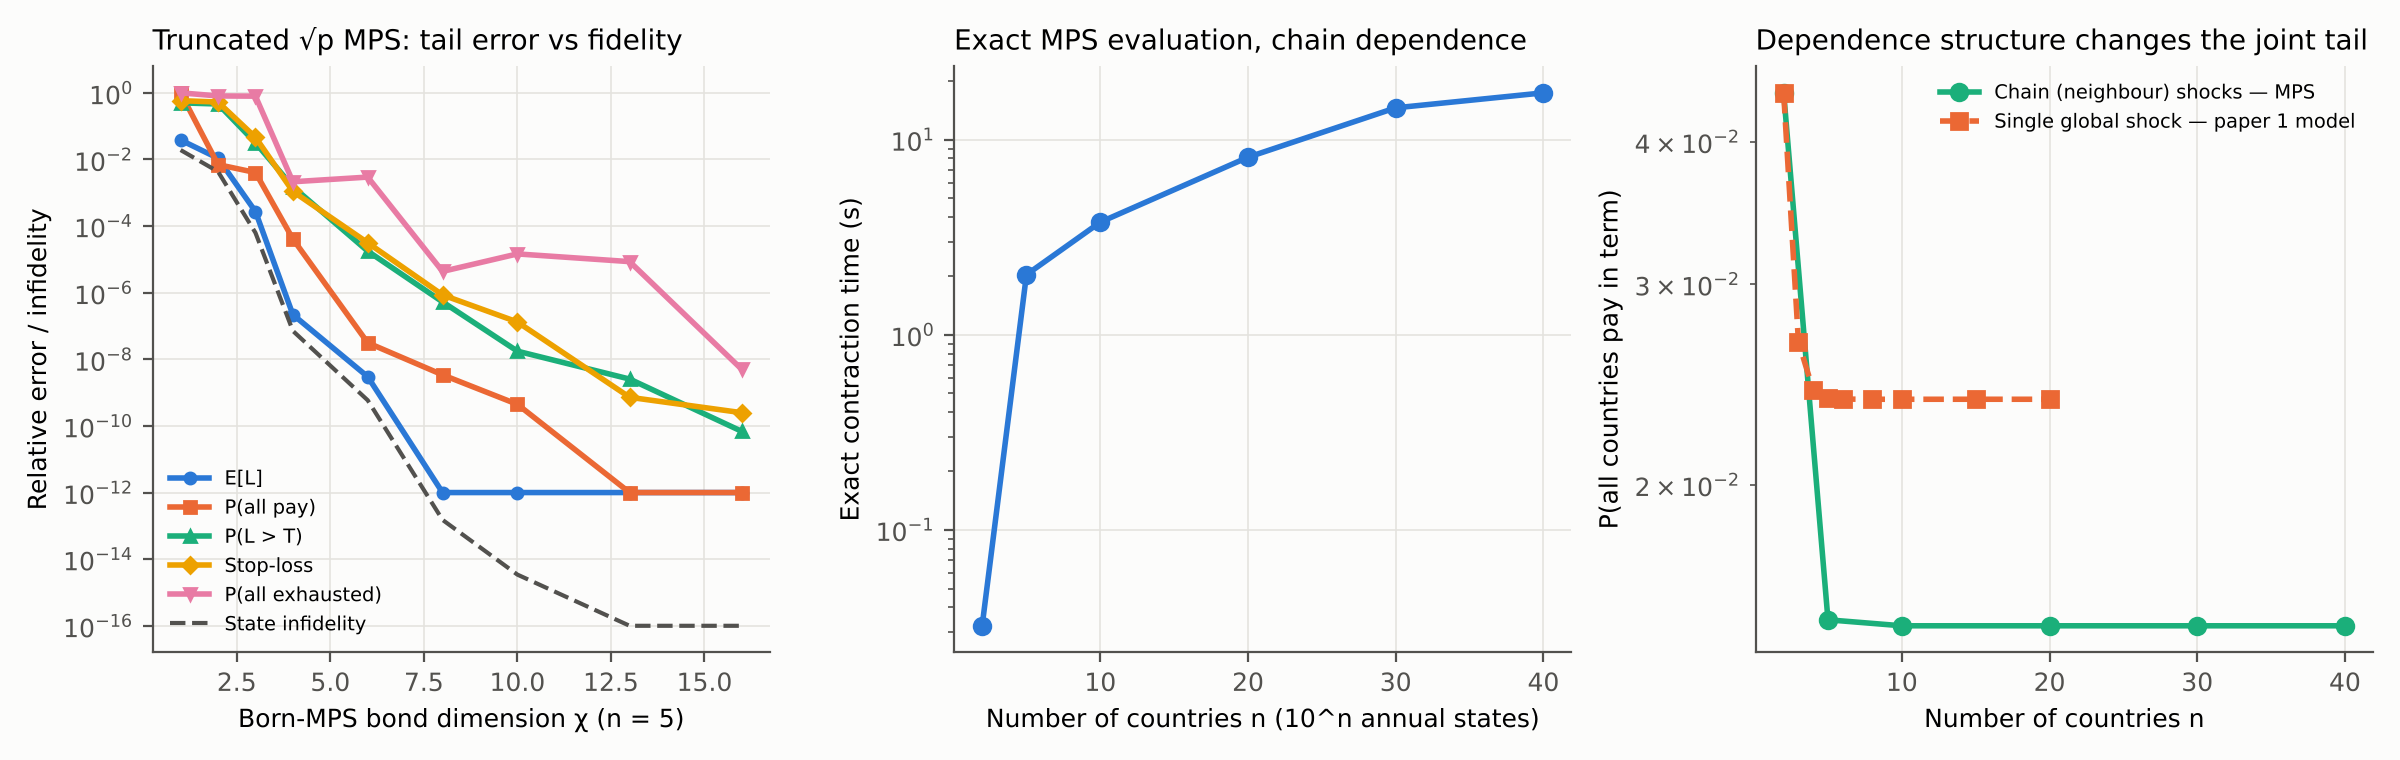
\includegraphics[width=\textwidth]{figures/fig_mps.png}
\caption{Left: relative error of each target and state infidelity versus Born-MPS bond dimension $\chi$ ($n=5$).
Centre: exact contraction time versus number of countries. Right: $\Pr(\text{all countries pay})$ for neighbour-coupled
shocks (this work) and a single global shock (companion paper~\cite{paper1}).}
\label{fig:mps}
\end{figure*}

\subsection{Discovered ranks}\label{sec:ranks}
Table~\ref{tab:ranks} lists the TT-SVD ranks. At $10^{-8}$ tolerance the ranks of $p$ are 7 and those of $\sqrt{p}$ at
most 13, and neither grows from $n=3$ to $n=5$. The constructed bond of 64 is therefore far from minimal, and the
distribution is intrinsically low-rank. The square root costs roughly twice the rank of $p$, because $\sqrt{\cdot}$
does not preserve the sum-of-products structure of~\eqref{eq:chain}.

\begin{table}[t]
\caption{TT-SVD ranks discovered without model knowledge}
\label{tab:ranks}
\centering\small
\begin{tabular}{rlll}
\toprule
$n$ & tolerance & ranks of $p$ & ranks of $\sqrt{p}$\\
\midrule
3 & $10^{-4}$ & [3, 3] & [5, 5]\\
3 & $10^{-8}$ & [7, 7] & [10, 10]\\
4 & $10^{-8}$ & [7, 7, 7] & [10, 13, 9]\\
5 & $10^{-4}$ & [4, 4, 4, 4] & [5, 6, 6, 5]\\
5 & $10^{-8}$ & [7, 7, 7, 7] & [10, 13, 13, 10]\\
\bottomrule
\end{tabular}
\end{table}

\subsection{Born-MPS loader: fidelity versus tail accuracy}\label{sec:born}
Table~\ref{tab:born} and Fig.~\ref{fig:mps} (left) show the effect of truncating $\sqrt{p}$ for $n=5$. State
infidelity falls quickly, but tail targets lag far behind: at $\chi=3$ the infidelity is $6.3\times10^{-5}$ while
$\Pr(\text{all exhausted})$ is wrong by $79\%$. Fidelity weighs states by $p$, so it barely registers states of
probability $10^{-9}$, which are exactly the ones that determine the exhaustion target. Truncation for risk
applications must therefore be chosen by tail-target error, not by fidelity or KL divergence. At $\chi=8$ every target
is within $4.4\times10^{-6}$ relative error; at $\chi=16$ within $5\times10^{-9}$.

\begin{table}[t]
\caption{Born-MPS truncation ($n=5$) and loader resources}
\label{tab:born}
\centering\small
\setlength{\tabcolsep}{2.8pt}
\begin{tabular}{rrrrrr}
\toprule
$\chi$ & $1-F$ & max rel.\ err. & exh.\ err. & qubits & CNOT/site\\
\midrule
2 & $4.3\times10^{-3}$ & 0.81 & 0.81 & 21 & 491\\
3 & $6.3\times10^{-5}$ & 0.79 & 0.79 & 22 & 1{,}963\\
4 & $7.1\times10^{-8}$ & $2.1\times10^{-3}$ & $2.1\times10^{-3}$ & 22 & 1{,}963\\
8 & $1.5\times10^{-13}$ & $4.4\times10^{-6}$ & $4.4\times10^{-6}$ & 23 & 7{,}851\\
16 & $<10^{-15}$ & $5.0\times10^{-9}$ & $5.0\times10^{-9}$ & 24 & 31{,}403\\
\bottomrule
\multicolumn{6}{l}{\footnotesize Qubits $=4n+\lceil\log_2\chi\rceil$; CNOT/site $=\lceil\tfrac{23}{48}4^{\lceil\log_2\chi\rceil+4}\rceil$ (generic bound).}
\end{tabular}
\end{table}

With $\chi=8$ and $n=40$ the loader needs $163$ qubits and about $3.1\times10^{5}$ CNOTs per call, using the generic
bound; structured site unitaries would reduce this. A generic preparation of the same state would need
$O(2^{4n})$ CNOTs. The loader thus keeps the QAE oracle linear in $n$ for dependence structures without a global
factor, which is the case left open by the companion paper~\cite{paper1}.

%=====================================================================
\section{Discussion}
%=====================================================================
\subsection{Where the quantum-inspired method stands}
For local dependence of bounded range, MPS contraction is exact and fast, so neither sampling nor QAE is needed:
the classical tensor network is the method of choice. This sharpens the question the challenge poses. A quantum
advantage can only arise for distributions whose MPS bond dimension grows quickly with $n$---for example, event sets
in which large footprints couple distant countries, or two-dimensional hazard fields. For those, a Born machine on a
quantum computer can represent correlations an MPS cannot hold efficiently, and QAE can then estimate the targets.
Measuring how bond dimension grows for realistic event sets is therefore the decisive experiment.

\subsection{Limitations}
\begin{itemize}
\item The chain model is synthetic; link rates reuse the ADB shared rate.
\item Poisson counts are truncated at three events per link-year; the induced error is reported and below $10^{-9}$
for $n\le40$.
\item Loader CNOT counts use a generic unitary bound and are not transpiled.
\item Born-MPS truncation was studied for $n\le5$, where the full tensor fits in memory; larger $n$ requires
TT-rounding directly on the cores.
\end{itemize}

%=====================================================================
\section{Phase~2 Plan}
%=====================================================================
\begin{table}[t]
\caption{Phase~2 plan}
\label{tab:plan}
\centering\small
\setlength{\tabcolsep}{3pt}
\begin{tabular}{p{0.09\columnwidth}p{0.55\columnwidth}p{0.27\columnwidth}}
\toprule
Weeks & Work & Gate / output\\
\midrule
1--3 & TT-rounding on cores; tail-aware truncation (minimise target error, not fidelity) & Bond vs.\ $n$ up to 100\\
4--6 & Event-set model with multi-country footprints (USGS- and NASA-GPM-informed); measure bond growth; 2-D (PEPS/tree) variants & Gate 1: is bond growth polynomial?\\
7--9 & Born-MPS circuits in a quantum SDK; transpiled depth; QAE on GPU simulators & Measured loader cost\\
10--12 & Compare MPS, QCBM~\cite{benedetti2019} and QAE end to end; report, code, demo & Gate 2: quantum claim or negative result\\
\bottomrule
\end{tabular}
\end{table}

Table~\ref{tab:plan} lists the plan. If bond dimension stays small for realistic event sets, the deliverable is a
classical tensor-network engine for ADB; if it grows, the Born-MPS loader and QAE become the candidate route, and
their cost is measured rather than assumed.

%=====================================================================
\section{Conclusion}
%=====================================================================
A matrix product state represents the ADB joint-loss benchmark exactly and extends it to neighbour-coupled
dependence, which single-factor methods cannot handle. Exact contraction evaluates portfolios of 40 countries and
targets as small as $10^{-55}$ in seconds. The distribution is intrinsically low-rank, and its square root yields a
Born-machine loader for QAE with linear cost in $n$. Tail targets, not fidelity, must govern truncation.

\section*{Team}
\todo{Members, roles, and relevant experience.}

\section*{Reproducibility and Use of AI}
Code and results are in the accompanying package; all numbers are produced by deterministic scripts in about one
minute on a two-core CPU (Python 3.13, NumPy 2.5, SciPy 1.18). \todo{Describe the team's use of AI tools.}

\begin{thebibliography}{00}
\bibitem{brief} Asian Development Bank, ``Quantum approaches to joint-loss modelling for natural catastrophe risk,'' Challenge Description, ADB Quantum Innovation Challenge, 2026.
\bibitem{adbbond} Asian Development Bank, ``ADB issues inaugural disaster relief bonds targeting earthquake and extreme precipitation risk in the Kyrgyz Republic and Tajikistan,'' News release, May 3, 2026.
\bibitem{paper1} \todo{Companion submission}, ``Quantum amplitude estimation for joint catastrophe-bond risk: An exact benchmark study on the ADB Kyrgyz--Tajik disaster relief bonds,'' 2026.
\bibitem{orus2014} R. Or\'us, ``A practical introduction to tensor networks: Matrix product states and projected entangled pair states,'' \emph{Ann. Phys.}, vol. 349, pp. 117--158, 2014.
\bibitem{oseledets2011} I. V. Oseledets, ``Tensor-train decomposition,'' \emph{SIAM J. Sci. Comput.}, vol. 33, no. 5, pp. 2295--2317, 2011.
\bibitem{han2018} Z.-Y. Han, J. Wang, H. Fan, L. Wang, and P. Zhang, ``Unsupervised generative modeling using matrix product states,'' \emph{Phys. Rev. X}, vol. 8, art. 031012, 2018.
\bibitem{schon2005} C. Sch\"on, E. Solano, F. Verstraete, J. I. Cirac, and M. M. Wolf, ``Sequential generation of entangled multiqubit states,'' \emph{Phys. Rev. Lett.}, vol. 95, art. 110503, 2005.
\bibitem{shende2006} V. V. Shende, S. S. Bullock, and I. L. Markov, ``Synthesis of quantum-logic circuits,'' \emph{IEEE Trans. Comput.-Aided Des. Integr. Circuits Syst.}, vol. 25, no. 6, pp. 1000--1010, 2006.
\bibitem{brassard2002} G. Brassard, P. H{\o}yer, M. Mosca, and A. Tapp, ``Quantum amplitude amplification and estimation,'' \emph{Contemp. Math.}, vol. 305, 2002.
\bibitem{montanaro2015} A. Montanaro, ``Quantum speedup of Monte Carlo methods,'' \emph{Proc. R. Soc. A}, vol. 471, 2015.
\bibitem{benedetti2019} M. Benedetti \emph{et al.}, ``A generative modeling approach for benchmarking and training shallow quantum circuits,'' \emph{npj Quantum Inf.}, vol. 5, art. 45, 2019.
\end{thebibliography}

\end{document}
